\documentclass{iopart}
\usepackage{arydshln}
\usepackage{multirow}
\usepackage{amsopn}
\usepackage{iopams}
\usepackage{graphicx}
\usepackage{bib/aas_macros}
\usepackage[colorlinks]{hyperref}
\input{ligo-acronyms/acronyms}

% From http://www.f.kth.se/~ante/latex.php
\setlength{\marginparwidth}{1.2in}
\let\oldmarginpar\marginpar
\renewcommand\marginpar[1]{\-\oldmarginpar[\raggedleft\footnotesize #1]%
{\raggedright\footnotesize #1}}

\DeclareMathOperator{\cov}{cov}
\DeclareMathOperator{\std}{std}

\begin{document}

\title[Rapid-response Bayesian sky localization]{Rapid-response Bayesian sky localization for electromagnetic follow-up of gravitational-wave candidates}
\author{Leo Singer and Larry R. Price}
\address{\acs{LIGO} Laboratory, California Institute of Technology, Pasadena, CA 91125, USA}
\ead{\mailto{leo.singer@ligo.org}, \mailto{larryp@caltech.edu}}

\begin{abstract}
Timely \acl{EM} follow\nobreakdashes-up of \acl{CBC} events detected by \acl{aLIGO} requires rapidly inferring the sky location from the \ac{GW} observations. Calculation of the posterior distribution of the sky location and intrinsic source parameters given the \ac{GW} strain takes hours with state\nobreakdashes-of\nobreakdashes-the\nobreakdashes-art \ac{MCMC} parameter estimation codes. By taking as the measurement not the \ac{GW} strain itself but the amplitude and \acl{TOA} of the putative signal at each detector, and by fixing the intrinsic source parameters, we have constructed a non-\ac{MCMC}, fully deterministic Bayesian parameter estimation algorithm that takes just seconds to produce sky maps of posterior probability.%
\marginpar{Wrong emphasis? I like Larry's idea of having this paper discuss several different tiers of sky localization with increasing accuracy and latency.}
\end{abstract}

\section{Outline}

\begin{enumerate}
\item Introduction {
	\begin{enumerate}
	\item Background: \acp{GRB}, \acp{CBC}, \acs{LIGO}
	\item Time scales of \acp{GRB}, \acp{CBC}
	\item Current sky localization algorithms and response times
	\end{enumerate}
}
\item Preliminaries {
	\begin{enumerate}
	\item Fisher information, \ac{CRLB}
	\item Matched\nobreakdashes-filter estimator
	\end{enumerate}
}
\item Algorithm {
	\begin{enumerate}
	\item Assumptions
	\item Signal model
	\item Likelihood function
	\item Priors and marginalization
	\item Procedure
	\end{enumerate}
}
\item Results {
	\begin{enumerate}
	\item Injection population
	\item Cumulative fraction vs. confidence level plots
	\item Sky localization accuracy as a function of distance or \ac{SNR}
	\item Speed
	\end{enumerate}
}
\item Discussion {
	\begin{enumerate}
	\item Potential further refinements
	\item What astrophysical targets were accessible before
	\item What new targets are available with the response time of seconds
	\item Lay out timeline of follow\nobreakdashes-up campaign, including different tiers of inference and different types of telescopes
	\end{enumerate}
}
\item Appendices {
	\begin{enumerate}
	\item Code listing?
	\item Any proofs that are needed in the body but would interrupt the text?
	\end{enumerate}
}
\end{enumerate}


\section{Introduction}

Ground-based \ac{GW} interferometers are entering the advanced detector era, positioning themselves to make profound discoveries about the universe. The \ac{aLIGO} and Vigo detectors will be part of a worldwide network that also includes KAGRA and hopefully LIGO-India. Coalescing neutron star binaries are among the most likely sources, with event rates of $~ 50/\mathrm{yr}$~\cite{rates}.%
%
\marginpar{Check that number.}
%
In addition to being an efficient source of \acp{GW}, the \ac{NS} may be tidally shredded before merging, providing fuel for an electromagnetic counterpart. The short-lived accretion flow may power a collimated relativistic jet, resulting in a short \ac{GRB} and an X-ray afterglow if it is aligned with the line of sight. An optical afterglow may follow minutes to hours later as the jet plows into the interstellar medium. As surrounding neutron-rich ejecta decay radioactively, an optical `kilonova' may be visible after $\sim$1 day \cite{metzger:2010}. Finally, as the ejecta plow into the interstellar medium, a faint radio afterglow could occur on a timescale of weeks to years \cite{Nakar:2011cw}.

There is therefore a strong case for performing electromagnetic followups of these sources of \acp{GW}. Indeed, the final science run of the intitial LIGO and Virgo instruments saw the first joint search for \acp{GW} from compact binaries and their electromagnetic counterparts \cite{abadie2012first}.  As we prepare for the next generation of these searches there is a need for determining the location of the source as precisely as possible in as little time as possible.

In this paper we present a rapid and accurate method of sky localization that makes use of Bayesian methods. It differs from existing techniques is several important ways.  In the first place, we fix the intrinsic parameters to their maximum likelihood estimates, as provided by the detection pipeline.  This reduces the dimensionality of the parameter we need to search. In addition, the technique takes as its input the maximum likelihood estiamtes of the extrinsic parameters, instead of the $h(t)$ time series. This makes the likelihood itself much faster to evaluate. Finally, instead of of using \ac{MCMC} or some similar method for statistical sampling, we make use of a deterministic quadrature scheme. We call this technique \ac{BAYESTAR}%
%
\footnote{A pun on the Cylon battleships in the American television series Battlestar Galactica. The defining characteristic of the Cylons is that they repeatedly defeat humanity by using their superhuman information\nobreakdashes-gathering ability to coordinate overwhelming forces. The name also suggests that, like the Cylons, \acp{GW} detectors may some day rise against us humans.}%
%
\footnote{We do not like to mention the final `T' in the acronym, because then it would be called BAYES\nobreakdashes-TART, which would sound ridiculous.}%
.

\section{Setup}

A laser interferometer senses \acp{GW} by transducing differential changes in arm length to a digitized photocurrent time series. In the angular frequency domain, a single detector's observation $X_i(\omega)$ is
%
\begin{equation}\label{eq:signal-model}
	X_i (\omega) = H_i (\omega; \boldsymbol\theta) + N_i (\omega),
\end{equation}
%
where $H_i (\omega; \boldsymbol\theta)$ is the \ac{GW} signal receied by detector $i$, given a parameter vector $\boldsymbol\theta$ that describes the \ac{GW} source, and $N_i (\omega)$ is that detector's \ac{WSS} Gaussian noise with \ac{PSD} $S_i(\omega)$. We shall denote the combined observation from a network of detectors as $\mathbf X (\omega) \equiv \{X_i (\omega)\}_i$.

The likelihood, or the probability of obtaining the observation $\mathbf X$ conditioned on the value of $\boldsymbol\theta$, is Gaussian, with the log\nobreakdashes-likelihood proportional to:
%
\begin{equation}\label{eq:gaussian-likelihood}
	\mathcal{L}(\mathbf X; \boldsymbol\theta) = \prod_i p(X_i | \boldsymbol\theta)
		\propto \exp \left[
		- \frac{1}{2} \sum_i \int_0^\infty \frac{\left|X_i (\omega)
			- H_i(\omega; \boldsymbol\theta) \right|^2}{S_i(\omega)} \, \mathrm{d}\omega
	\right].
\end{equation}

A \ac{CBC} source is specified by a vector of extrinsic parameters describing its position and orientation and intrinsic parameters describing the physical properties of the binary components:
%
\begin{equation}
    \boldsymbol\theta = \begin{array}{l@{}l}
            \left[
            \begin{array}{c}
                \alpha \\
                \delta \\
                D_\mathrm{L} \\
                t_\oplus \\
                \iota \\
                \psi \\
                \phi_c \\
                \hdashline[1pt/1pt]
                m_1 \\
                m_2 \\
                \mathbf S_1 \\
                \mathbf S_2
            \end{array}
            \right] &
            \begin{array}{l}
                \left.
                \begin{array}{p{4cm}}
                    right ascension \\
                    declination \\
                    luminosity distance \\
                    arrival time at geocenter \\
                    inclination angle \\
                    polarization angle \\
                    coalescence phase \\
                    \hdashline[1pt/1pt]
                \end{array}
                \quad \right\} \textnormal{extrinsic parameters}, \boldsymbol\theta_\mathrm{ex} \\
                \left.
                \begin{array}{p{4cm}}
                    first component's mass \\
                    second component's mass \\
                    first component's spin \\
                    second component's spin
                \end{array}
                \quad \right\} \textnormal{intrinsic parameters}, \boldsymbol\theta_\mathrm{in}
            \end{array}
        \end{array}
\end{equation}
%
Binary eccentricity is omitted as an intrinisc parameter because tidal interaction of the progenitor stars~\cite{0004-637X-572-1-407} and later \ac{GW} emission~\cite{PhysRev.136.B1224} circularize the orbit long before the inspiral enters \ac{LIGO}'s frequency range of $\sim$10\nobreakdashes--1000~kHz. Tidal deformabilities of the \acp{NS} are omitted because the effect of tides on the inspiral would only be detectable by an Einstein Telescope-class \ac{GW} observatory~\cite{PhysRevD.81.123016}. Furthermore, in \ac{GW} detection efforts, especially those focused on \ac{NSNS} systems, the component spins $\mathbf{S}_1$ and $\mathbf{S}_2$ are often assumed to be aligned with the system's total angular momentum and condensed to a single scalar parameter $\chi$, or even neglected entirely, $\mathbf{S}_1 = \mathbf{S}_2 = 0$. In this work we will consider only zero spin.

Assuming circular orbits and no spin precession, we can write the \ac{GW} signal in each detector as a linear combination of two basis waveforms $H_0$ and $H_{\pi/2}$. For nonprecessing systems, $H_0$ and $H_{\pi/2}$ are approximately ``in quadrature'' in the same sense as the sine and cosine functions, being nearly orthogonal and out of phase by ${\pi/2}$ at all frequencies. In other words, $H_{\pi/2}(\omega) = i H_0(\omega)$ for all $\omega$. This linear combination isolates all dependence on the extrinsic parameters $\boldsymbol\theta_\mathrm{ex}$ into the coefficients and all dependence on the intrinsic parameters $\boldsymbol\theta_\mathrm{in}$ into the basis waveform,
%
\begin{eqnarray}
	\fl H_i(\omega; \boldsymbol\theta) &=& e^{-i\omega t_\oplus}\frac{D_{1,i}}{D_\mathrm{L}}
	\left(\begin{array}{cc}
		F_{+,i}(h_i, \delta) \\
		F_{\times,i}(h_i, \delta)
	\end{array}\right)^\intercal
	\left(\begin{array}{cc}
		\cos{2\psi} & -\sin{2\psi} \\
		\sin{2\psi} & \cos{2\psi}
	\end{array}\right)
	\left(\begin{array}{cc}
		\frac{1}{2}\left(1+\cos^2{\iota}\right) & 0 \\
		0 & \cos{\iota}
	\end{array}\right) \nonumber\\\fl &\cdot&
	\left(\begin{array}{cc}
		\cos{2\phi_c} & -\sin{2\phi_c} \\
		\sin{2\phi_c} & \cos{2\phi_c}
	\end{array}\right)
	\left(\begin{array}{cc}
		1 \\
		\imath
	\end{array}\right) H_0(\omega; \boldsymbol\theta_\mathrm{in}).
\end{eqnarray}
%
This linear combination matches the conventions used in \cite{PhysRevD.83.084002}, and is the frequency-domain equivalent of their Equation~(2.8). The quantities $F_{+,i}$ and $F_{\times,i}$ are the dimensionless detector antenna factors, and depend on the orientation of detector $i$ as well as the declination and local hour angle $h_i$ of the source, and are derived in~\cite{PhysRevD.63.042003}. The quantity $D_{1,i}$ is a fiducial horizon distance for detector $i$.

In the Bayesian framework, the parameters are inferred from the data by forming the posterior distribution, $p(\boldsymbol\theta|\mathbf X)$, which describes the probability of the parameters given the observations. Bayes' rule relates the likelihood $p(\mathbf X|\boldsymbol\theta)$ to the posterior $p(\boldsymbol\theta|\mathbf X)$,
%
\begin{equation}\label{bayes}
p(\boldsymbol\theta|\mathbf X) = \frac{p(\mathbf X|\boldsymbol\theta) p(\boldsymbol\theta)}{p(\mathbf X)},
\end{equation}
%
introducing the prior distribution $p(\boldsymbol\theta)$ which encapsulates previous information about the paramters (for example, arising from earlier observations or from known physical bounds on the parameters), and the evidence $p(\mathbf X)$ which can be thought of as a normalization factor or as describing the parsimoniousness of the model.

Removing nuisance parameters requires either replacing them with their measured values or marginalizing over them. The chirp mass is typically well measured by the detection pipeline, so we use the maximum likelihood value, $\hat{\mathcal{M}}$, for it. We marginalize over the other variables using a uniform prior, i.e.,
%
\begin{equation}
p(\alpha,\delta,D_L|d) = \int\, d\tau_\oplus p_U(\tau_\oplus) d\phi_c p_U(\phi_c) d\phi p_U(\psi)  d\cos(\iota) p_U(\cos(\iota)) p(\alpha,\delta,D_L,\tau_\oplus,\phi_c,\psi,\cos(\iota)|d),
\end{equation}
%
where $p_U(x)$ denotes a uniform distribution in $x$.

For typical parameter estimation studies, the data, $d$, is taken to be the strain time series in each detector, $h_I(t)$, where $I$ indexes the detectors. Our interest here, however, is in obtaining accurate sky location results as quickly as possible. To that end, we instead base our posteriors on the maximum likelihood estimates of the signal-to-noise ratio (SNR), $\hat{\rho}_I$, the time-of-arrival (TOA), $\hat{\tau}_I$, and coalescence phase, $\hat{\phi}_I$, measured in each detector by the detection pipeline. Thus the sky location posterior can be computed without any re-filterning of the data.

\section{Measurement uncertainty}

The \ac{CRLB} is a useful analytical tool for predicting with what error an unknown parameter or parameters can be estimated from noisy observations. When an unbiased estimator exists, the \ac{CRLB} bound says that the covariance of the estimation error is bounded below by the Fisher information matrix. The \ac{CRLB} has been widely applied in \ac{GW} astronomy, for instance by \cite{fairhurst:2009} to predict the sky localization accuracy that is achievable with \ac{GW} observations. Here, we review the Fisher matrix calculation in \cite{fairhurst:2009} but add some physical interpretation to the particular structure of the covariance matrix.

\subsection{Fisher matrix}

In the frequency domain, the strain $X (\omega)$ observed by a detector is a linear combination of two orthogonal \ac{GW} quadratures and additive noise,
%
\begin{equation}\label{eq:signal-model}
	X (\omega) = H (\omega, \rho, \gamma, \tau) + N (\omega) = \frac{\rho}{\sigma} e^{\imath (\gamma - \omega \tau)} U (\omega) + N (\omega),
\end{equation}
%
where $H (\omega)$ is the signal content, $N (\omega)$ is the detector's \ac{WSS} Gaussian noise with \ac{PSD} $S(\omega)$, $U (\omega)$ is the frequency-domain post-Newtonian inspiral signal, $\rho$ is the signal's amplitude, $\gamma$ is a phase angle the encodes the relative strength of two \ac{GW} quadratures, and $\tau$ is the time of arrival relative to an arbitrary time base. The quantity $\sigma$ is a normalization constant defined as the \ac{SNR} of the \ac{GW} source at a fiducial distance, here taken to be $D_\mathrm{fiducial} = 1$~Mpc,
%
\begin{equation}\label{eq:sigma}
    \sigma^2 = \int_0^\infty \frac{\left| U (\omega)\right|^2}{S(\omega)} \, \mathrm{d}\omega.
\end{equation}
%
The distance at which an optimally oriented \ac{GW} source would produce \ac{SNR}=1 is defined as $D_1 = D_\mathrm{fiducial} / \sigma$. The likelihood, or the probability of obtaining the observation $X(\omega)$ conditioned on the value of the parameter vector $\boldsymbol\theta = (\rho, \gamma, \tau)$, is Gaussian, with the log-likelihood proportional to:
%
\begin{equation}\label{eq:gaussian-likelihood}
	\mathcal{L}(X; \boldsymbol\theta) = p(X | \boldsymbol\theta)
		\propto \exp \left[
		- \frac{1}{2} \int_0^\infty \frac{\left|X (\omega)
			- H(\omega; \boldsymbol\theta) \right|^2}{S(\omega)} \, \mathrm{d}\omega
	\right].
\end{equation}

The Fisher information matrix for a measurement $\tilde x$ described by the unknown parameter vector $\boldsymbol{\theta}$ is
%
\begin{equation}\label{eq:general-fisher-matrix}
	\mathcal{I}_{jk} = \mathrm{E} \, \left[
		-\frac{\partial^2 \log
			\mathcal{L}(X ; \boldsymbol\theta)}
			{\partial \theta_j \theta_k}
	\right].
\end{equation}
%
This equation involves double derivatives, but substantial simplification is possible when---as in this case---the likelihood is Gaussian:
%
\begin{equation}\label{eq:gaussian-fisher-matrix}
	\mathcal{I}_{jk} = \int_0^\infty \Re \left[
        \left(\frac{\partial H}{\partial \theta_j}\right)^*
        \left(\frac{\partial H}{\partial \theta_k}\right)
	\right] \frac{1}{S(\omega)} \, \mathrm{d}\omega.
\end{equation}
%
This form is more useful because it involves only first derivatives, and of the signal $\tilde h (\omega)$ rather than the entire observation $\tilde x (\omega)$. In terms of the $k$th \ac{SNR}-weighted moment of angular frequency,
%
\begin{equation}\label{eq:angular-frequency-moments}
    \overline{\omega^k} =
        \left[ \int_0^\infty \frac{|U (\omega)|^2}{S(\omega)} \omega^k \, \mathrm{d}\omega \right]
        \left[ \int_0^\infty \frac{|U (\omega)|^2}{S(\omega)} \, \mathrm{d}\omega \right]^{-1},
\end{equation}
%
the Fisher matrix for the signal model in \Eref{eq:signal-model} is
%
\begin{equation}\label{eq:fisher-matrix}
	\mathcal{I} = \bordermatrix{
        ~ & \rho & \gamma & \tau \cr
        \rho & 1 & 0 & 0 \cr
        \gamma & 0 & \rho^2 & -\rho^2 \overline{\omega} \cr
        \tau & 0 & -\rho^2 \overline{\omega} & \rho^2 \overline{\omega^2}
    }.
\end{equation}

\subsection{\ac{CRLB} and physical interpretation}

The \ac{CRLB} says that, element by element,
%
\begin{equation}\label{eq:covariance-matrix}
    \cov{
        \left(
        \begin{array}{c}
            \hat{\rho} - \rho \\
            \hat{\gamma} - \gamma \\
            \hat{\tau} - \tau
        \end{array}
        \right)
    } \geq \mathcal{I}^{-1} = \left(
        \begin{array}{ccc}
            1 & 0 & 0 \\
            0 & \rho^2 \overline{\omega^2}/{\omega_\mathrm{rms}}^2 & \rho^2 \overline{\omega}/{\omega_\mathrm{rms}}^2 \\
            0 & \rho^2 \overline{\omega}/{\omega_\mathrm{rms}}^2 & \rho^2/{\omega_\mathrm{rms}}^2
        \end{array}
    \right)
\end{equation}
%
where a hat $\hat{\phantom{\rho}}$ denotes the estimate of a parameter and ${\omega_\mathrm{rms}}^2 = \overline{\omega^2} - \overline{\omega}^2$. Reading off the $\tau \tau$ element of the covariance matrix reproduces the timing accuracy in Equation~(24) of \cite{fairhurst:2009},
%
\begin{equation}\label{eq:timing-crlb}
    \std \left(\hat{\tau} - \tau \right) \geq \sqrt{\left(\mathcal{I}^{-1}\right)_{\tau\tau}} = \frac{\rho}{\omega_\mathrm{rms}}.
\end{equation}

\marginpar{Plot covariance ellipses and estimator samples for each change of variables; that would be a nice visual here.}%
%
Furthermore, the Fisher matrix in \Eref{eq:fisher-matrix} is block diagonal, which implies that estimation errors in the signal amplitude $\rho$ are uncorrelated with the phase $\gamma$ and time $\tau$. A sequence of two changes of variables lends some physical interpretation to the nature of the coupled estimation errors in $\gamma$ and $\tau$.

First, we put the phase and time on the same footing by measuring the time in units of $1 / 2 \pi \sqrt{\overline{\omega^2}}$ with a change of variables from $\tau$ to $\gamma_\tau = 2 \pi \sqrt{\overline{\omega^2}} \tau$:
%
\begin{equation}
    \mathcal{I}' = \bordermatrix{
        ~ & \rho & \gamma & \gamma_\tau \cr
        \rho & 1 & 0 & 0 \cr
        \gamma & 0 & \rho^2 & -\rho^2\frac{\overline{\omega}}{\sqrt{\overline{\omega^2}}} \cr
        \gamma_\tau & 0 & -\rho^2\frac{\overline{\omega}}{\sqrt{\overline{\omega^2}}} & \rho^2
    }.
\end{equation}

The second change of variables, from $\gamma$ and $\gamma_\tau$ to $\gamma_\pm = \frac{1}{\sqrt{2}}(\gamma \pm \gamma_\tau)$, diagonalizes the Fisher matrix:
%
\begin{equation}
    \mathcal{I}'' = \bordermatrix{
        ~ & \rho & \gamma_+ & \gamma_- \cr
        \rho & 1 & 0 & 0 \cr
        \gamma_+ & 0 & \left(1 - \frac{\overline{\omega}}{\sqrt{\overline{\omega^2}}}\right)\rho^2 & 0 \cr
        \gamma_- & 0 & 0 & \left(1 + \frac{\overline{\omega}}{\sqrt{\overline{\omega^2}}}\right)\rho^2
    }.
\end{equation}
%
Thus, in the appopriate time units, the \textit{sum and difference} of the phase and time of the signal are measured independently.

\subsection{Noise model for point parameters}

The likelihood in \Eref{eq:gaussian-likelihood} is the quantity that is maximized by the matched\nobreakdashes-filter estimator. However, just because we have the covariance matrix defined by \Eref{eq:covariance-matrix} does not mean that the distribution of estimator errors is multivariate Gaussian. Nonetheless, it is straightforward to qualitatively describe the distribution.

If we were to suppress the time parameter $\tau$, then we could reduce the likelihood to the form
%
\begin{equation}
    \mathcal{L}(z; \rho, \gamma) \propto \exp \left[ -\frac{1}{2} \left|z - e^{\imath \gamma} \rho \right|^2 \right]
\end{equation}
%
for a complex scalar measurement $z$. This likelihood also describes the distribution of the length $\rho$ and angle $\gamma$ of a vector whose Cartesian components are perturbed with normally distributed errors. For this problem, $\rho$ and $\gamma$ are uncorrelated, $\rho^2$ being noncentrally $\chi^2$\nobreakdashes-disributed with two degrees of freedom and $\gamma$ being von~Mises\nobreakdashes-distributed.
%
\marginpar{Picture here?}

\marginpar{What about if we suppress $\gamma$ or $\rho$? Do those cases teach us anything?}
%
We know that the matched\nobreakdashes-filter estimator's distribution, given a particular true value of $\rho$, $\gamma$, and $\tau$, must go to zero at $\hat{\rho}=0$ and must be periodic in $\gamma$ but not $\tau$. From just these properties, the estimator's distribution should be an approximate Gaussian, but wrapped diagonally around a cylinder where the radius represents $\hat{\rho}$, the angle around the cylinder represents $\hat{\gamma}$, and the distance up or down the cylinder represents $\hat{\tau}$.

There are many ways to realize distribution function with these properties, but they tend to be difficult to work with.
%
\marginpar{Give some examples.}
%
An alternative is to just discard the one periodic parameter, $\gamma$, entirely. We do not know the exact distribution of the remaining parameters $\rho$ and $\tau$, but we are less liable to make egregious errors by assuming that they are Gaussian than if we assumed that the estimation errors in $\gamma$ were Gaussian. Projecting out $\gamma$ gives us the covariance matrix
%
\begin{equation}
    \cov \left(
        \begin{array}{c}
            \hat{\rho} - \rho \\
            \hat{\tau} - \tau
        \end{array}
    \right) =
    \left(
        \begin{array}{cc}
            1 & 0 \\
            0 & \rho^2/{\omega_\mathrm{rms}}^2
        \end{array}
    \right).
\end{equation}

A wrinkle is that this covariance matrix still depends on the true, unknown value of $\rho$. If we make the further leap of evaluating the \ac{CRLB} \emph{at the value of the estimators}, we can then write the distribution of the estimator error as
%
\begin{eqnarray}
    \hat{\rho} - \rho \sim \mathcal{N}\, [0, 1] \\
    \hat{\tau} - \tau \sim \mathcal{N} \left[0, \hat{\rho}^2 / {\omega_\mathrm{rms}}^2\right],
\end{eqnarray}
%
valid at moderate to high \ac{SNR}.

\section{Method}

\subsection{Likelihood}

\marginpar{Explain why none of these expressions depend on the coalescence phase $\phi_c$.}%
%
If we assume that the time and amplitude estimation errors are uncorrelated, then we can separate the likelihood into one factor that depends only on time and one that depends only on amplitude:
%
\begin{eqnarray*}
    \mathcal{L}(
        \hat{\tau}_1, \hat{\tau}_2, &\dots, \hat{\tau}_N,
        \hat{\rho}_1, \hat{\rho}_2, \dots, \hat{\rho}_N;
        \mathbf{n}, t_\oplus, D_\mathrm{L}, x, \psi) \\
    &= \mathcal{L}_\mathrm{TOA}(
        \hat{\tau}_1, \hat{\tau}_2, \dots, \hat{\tau}_N; \mathbf{n}, t_\oplus) \\
        &\times
        \mathcal{L}_\mathrm{SNR}(\hat{\rho}_1, \hat{\rho}_2, \dots, \hat{\rho}_N;
         \mathbf{n}, D_\mathrm{L}, x, \psi
    ).
\end{eqnarray*}
%
The \ac{TOA}-only factor depends only on the \ac{TOA} estimates $\hat{\tau}_1, \hat{\tau}_2, \dots, \hat{\tau}_N$, the unknown sky location $\mathbf{n}$ (or equivalently, the right ascension $\alpha$, declination $\delta$, and sidereal time), and the absolute \ac{TOA} at an arbitrary reference point (herein, the geocenter), $t_\oplus$, the fixed geographical locations of the detectors, $\mathbf{r}_i$, and the speed of light $c$.
%
\begin{equation}
    \mathcal{L}_\mathrm{TOA} \propto
    \exp \left[
            -\frac{1}{2} \sum_{i=1}^N \frac{\left(\hat{\tau}_i - \tau_i\right)^2}{\left(\hat{\rho_i} / \omega_{\mathrm{rms},i}\right)^2}
        \right]
    = \exp \left[
        -\frac{1}{2} \sum_{i=1}^N \frac{\left(\hat{\tau}_i + \mathbf{n} \cdot \mathbf{r}_i / c - t_\oplus \right)^2}{\left(\hat{\rho_i} / \omega_{\mathrm{rms},i}\right)^2}
    \right]
\end{equation}
%
The \ac{SNR}-only factor depends only on the \ac{SNR} estimates $\hat{\rho}_1, \hat{\rho}_2, \dots, \hat{\rho}_N$, but it depends on the unknown sky location, luminosity distance $D_\mathrm{L}$, cosine-inclination $x = \cos \iota$, and polarization angle $\psi$.
%
\begin{equation}
    \mathcal{L}_\mathrm{SNR} \propto \exp \left[
        -\frac{1}{2} \sum_{i=1}^N \left(\hat{\rho}_i - \rho_i(\mathbf{n}, D_\mathrm{L}, x, \psi) \right)^2
    \right]
\end{equation}
%
\marginpar{Cite \ac{GRB} prospects paper appendix; a very similar equation appears there. Is there somewhere else that has this formula? Shutz doesn't, and Finn \& Chernoff's notation is too heavy.}%
%
It is easily shown that
%
\begin{eqnarray*}
    {\rho_i}^2 &=
        \frac{1}{8} \left(\frac{D_{1,i}}{D_\mathrm{L}}\right)^2 \left[
            ( {F_{+,i}}^2 + {F_{\times,i}}^2 \right)
            \left(1 + 6 x^2 + x^4 \right) \\
            &+ \left(1 - x^2 \right) \left( {F_{+,i}}^2 - {F_{\times,i}}^2 \right) \cos {2\psi}
            + 2 \left( {F_{+,i}} {F_{\times,i}} ) \sin {2\psi}
        \right],
\end{eqnarray*}
%
where $F_{+,i}$ and $F_{\times,i}$ are the `$+$' and `$\times$' antenna factors of detector $i$, themselves functions of sky location $\mathbf{n}$.

\subsection{Prior}

Prior is uniform in $\mathbf{n}$, $t_\oplus$, x, and $\psi$. For distance, can choose either a prior that is uniform in $\log D_\mathrm{L}$ or uniform in volume.

\subsection{Marginalization}

The overall arrival time $t_\oplus$ can be marginalized out analytically, giving the \ac{TOA}-only marginal posterior
%
\begin{equation}
    p(\mathbf{n} | \hat{\tau}_1, \hat{\tau}_2, \dots, \hat{\tau}_N) \propto \exp\left[
        -\frac{1}{2} \sum_{i=1}^N \frac{\left( \tilde{\tau}_i - \langle \tilde{\tau} \rangle \right)^2}{\left(\hat{\rho_i} / \omega_{\mathrm{rms},i}\right)^2}
    \right]
\end{equation}
%
where
%
\begin{equation}
    \langle \tilde{\tau} \rangle =
    \left(\sum_{i=1}^N \frac{{\tilde{\tau}_i}^2}{\left(\hat{\rho_i} / \omega_{\mathrm{rms},i}\right)^2}\right)\left(\sum_{i=1}^N \frac{1}{\left(\hat{\rho_i} / \omega_{\mathrm{rms},i}\right)^2}\right)^{-1}.
\end{equation}

The marginalization over $D_\mathrm{L}$, $x$, and $\psi$ must be done numerically. The outermost integration is over x and $\psi$, and is done with Newton--Cotes by evaluating $\mathcal{L}_\mathrm{SNR}$ on a regular lattice in $x$ and $\psi$. This integration scheme is first order in $x$ and second order in $\psi$.

\marginpar{Explain initial integration breakpoints and how they are calculated. Cite \texttt{gsl\_integrate\_qagp}.}%
%
The innermost integration is over $D_\mathrm{L}$ and is performed using adaptive Gaussian quadrature, but with a twist that speeds up convergence.

\begin{figure}
    \caption{\label{fig:radial_integrand}Illustration of initial subdivisions for radial integration scheme.}
    \begin{center}
        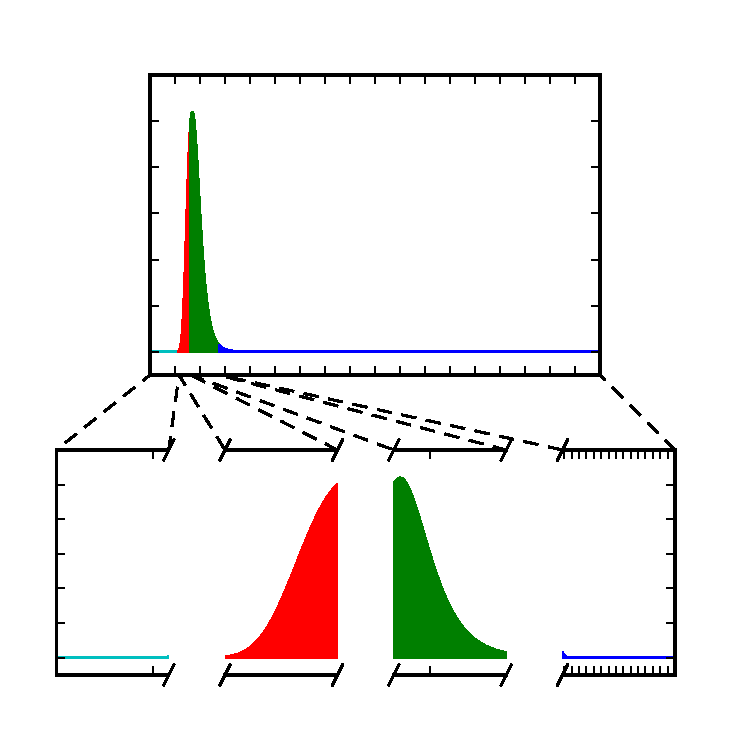
\includegraphics{radial_integrand}
    \end{center}
\end{figure}

\section{Hierarchical refinement}

\marginpar{Talk about adaptive selection of HEALPix resolution and of pixels on which to evaluate \ac{SNR} marginal posterior. Something to think about: this is logically easier to explain last, but chronologically makes more sense first.}


\ack Source code for \ac{BAYESTAR} is available on the \ac{LIGO} \acl{DASWG} web site at \url{http://www.lsc-group.phys.uwm.edu/daswg/projects/bayestar.html}.

Some of the results in this paper have been derived using HEALPix \cite{healpix}.

\ac{LIGO} was constructed by the California Institute of Technology and Massachusetts Institute of Technology with funding from the \ac{NSF} and operates under cooperative agreement PHY\nobreakdashes-0107417. Some results were produced on the NEMO computing cluster operated by the Center for Gravitation and Cosmology at University of Wisconsin\nobreakdashes--Milwaukee under \ac{NSF} Grants PHY\nobreakdashes-0923409 and PHY\nobreakdashes-0600953. This research is supported by the \ac{NSF} through a Graduate Research Fellowship to L.S. This paper has \ac{LIGO} Document Number \ac{LIGO}\nobreakdashes-PXXXXXXX\nobreakdashes-vX.


\section*{References}
\bibliographystyle{iopart-num}
\bibliography{apj-jour,bib/telescope}

\end{document}
